\documentclass[11pt,a4paper]{article}
\usepackage[margin=2.5cm]{geometry}
\usepackage{graphicx}
\usepackage{booktabs}
\usepackage{amsmath}
\usepackage{hyperref}
\usepackage{xcolor}
\usepackage{float}
\usepackage{caption}
\usepackage{subcaption}
\usepackage[numbers]{natbib}
\usepackage{siunitx}

\hypersetup{
    colorlinks=true,
    linkcolor=blue!60!black,
    citecolor=blue!60!black,
    urlcolor=blue!60!black
}

\graphicspath{{figures/}}

\title{Parametric vs Observational Salinity:\\
Validation of the SSWD-EvoEpi Seasonal Salinity Model\\
Against WOA23 Climatology}
\author{SSWD-EvoEpi Automated Analysis}
\date{March 2026}

\begin{document}
\maketitle

% ===================================================================
% 1. EXECUTIVE SUMMARY
% ===================================================================
\section{Executive Summary}

This report evaluates the parametric salinity baseline used in the SSWD-EvoEpi
disease model against monthly climatological surface salinity from the World
Ocean Atlas 2023 (WOA23) at 0.25\textdegree\ resolution, covering all 896
network nodes from 26.56\textdegree N (Baja California) to 61.19\textdegree N
(western Alaska).

The parametric model assigns each site a constant annual salinity based solely
on latitude:
\begin{equation}
S_{\text{ocean}}(\text{lat}) = 31.32 + 0.054 \times (\text{lat} - 50)
\label{eq:parametric}
\end{equation}
This formula captures the broad latitudinal gradient with a small overall mean
bias of $-0.13$~psu, but three critical deficiencies emerge:

\begin{enumerate}
    \item \textbf{Zero seasonal variation.} The parametric baseline produces
    exactly 0.00~psu seasonal range, whereas WOA23 shows a mean range of
    1.68~psu across all sites (max 8.11~psu in Prince William Sound). The model
    entirely misses seasonal freshening that drives disease suppression.

    \item \textbf{Large regional biases.} The monthly RMSE is 2.42~psu, with
    errors up to 9.18~psu. The model overestimates salinity by $+2.79$~psu in
    the Salish Sea (RMSE = 3.46~psu, $n=182$) and underestimates by $-2.50$~psu
    along the California coast (RMSE = 2.65~psu, $n=328$). The $R^2 = -0.32$
    for annual means, indicating the formula performs worse than simply using
    the global mean.

    \item \textbf{Wrong seasonal timing.} The month of minimum salinity varies
    widely: May (171 sites), June (152), February (116), and August (102).
    The parametric model's cosine melt pulse peaks on June~15 everywhere,
    missing the winter-storm freshening in California and late-glacial melt in
    Alaska.
\end{enumerate}

The disease-modelling consequences are stark. Under the parametric baseline,
\textbf{zero} of 896 sites experience any June salinity suppression (all values
$>30$~psu). Under WOA23, \textbf{143 sites} show $>1\%$ suppression, with
Salish Sea sites averaging 16.0\% and reaching 54.5\% suppression. The parametric
model is blind to this ecologically important signal.

We \textbf{recommend replacing the parametric baseline} with WOA23 monthly
climatology as the default salinity input.

% ===================================================================
% 2. DATA & METHODS
% ===================================================================
\section{Data Sources \& Methods}

\subsection{WOA23 Surface Salinity}

The World Ocean Atlas 2023 provides objectively analysed climatological mean
salinity on a 0.25\textdegree\ grid (approximately 20--28~km at these
latitudes). We extracted surface salinity (0~m depth) for all 12 calendar
months at each of the 896 SSWD-EvoEpi network nodes spanning from
113.15\textdegree W to 178.80\textdegree W.

Of the 896 sites, 235 (26.2\%) fall within a WOA23 ocean grid cell and receive
direct extraction. The remaining 661 (73.8\%) lie in WOA23 land cells ---
typically because these coastal and fjord sites sit inside the 0.25\textdegree\
land mask. For these, we used nearest-ocean-cell interpolation. The maximum
nearest-neighbour (NN) distance was 0.177\textdegree\ ($\approx$17~km), with a
mean of 0.094\textdegree\ ($\approx$9~km), indicating that the nearest ocean
cell is typically the immediately adjacent offshore grid cell.

\subsection{Parametric Baseline}

The current SSWD-EvoEpi model uses Equation~\ref{eq:parametric} to set ocean
salinity at each site. At \texttt{fw\_strength=0} (the baseline), this produces
a constant annual value per site with no seasonal cycle. The formula yields
values in a narrow band from 30.05~psu (26.56\textdegree N) to 31.92~psu
(61.19\textdegree N). By contrast, the WOA23 data span 22.14--34.31~psu ---
a 12~psu range compressed by the formula into less than 2~psu.

\subsection{Salinity Modifier for Disease Modelling}

The \textit{Vibrio} salinity modifier in the SSWD-EvoEpi model uses a nonlinear
transfer function:
\begin{equation}
S_{\text{mod}}(S) = \begin{cases}
0 & S \leq 10 \\
\left(\frac{S - 10}{28 - 10}\right)^{2} & 10 < S < 28 \\
1 & S \geq 28
\end{cases}
\label{eq:sal_mod}
\end{equation}
Salinity below 28~psu suppresses \textit{Vibrio} transmission; below 10~psu,
transmission ceases entirely. This nonlinear threshold means that even modest
salinity differences near 28~psu have disproportionate effects on predicted
disease dynamics.

\subsection{DFO Lighthouse Climatology}

As an independent validation, we compare both models against monthly salinity
climatologies from 12 Fisheries and Oceans Canada (DFO) lighthouse stations
along the British Columbia coast, representing decades of direct surface salinity
measurements at fixed coastal locations.

% ===================================================================
% 3. BASELINE COMPARISON
% ===================================================================
\section{Baseline Comparison}

\subsection{Annual Mean Scatter}

Figure~\ref{fig:scatter} compares parametric and WOA23 annual mean salinity
for all 896 sites. While the parametric model clusters tightly between
30.05--31.92~psu, WOA23 annual means span 22.14--34.31~psu. The scatter reveals
two dominant bias patterns:

\begin{itemize}
    \item \textbf{Salish Sea / WA} (green, $n=182$): The parametric model
    \emph{overestimates} salinity by $+2.79$~psu on average (RMSE = 3.46~psu).
    Northern Salish Sea sites (SS-N) show biases up to $+5.74$~psu because
    true estuarine salinities ($\sim$26~psu) are far below the parametric
    prediction.

    \item \textbf{OR / California} (red, $n=328$): The parametric model
    \emph{underestimates} by $-2.50$~psu (RMSE = 2.65~psu). These southern,
    open-ocean sites have true salinities of 33--34~psu, well above the formula's
    prediction.

    \item \textbf{British Columbia} (orange, $n=111$): Best agreement (bias =
    $+0.10$~psu, RMSE = 0.61~psu), expected since the formula was calibrated
    for BC conditions.

    \item \textbf{Alaska} (blue, $n=275$): Moderate positive bias ($+0.67$~psu,
    RMSE = 1.64~psu), with Prince William Sound (AK-PWS) a notable outlier
    (bias = $+2.29$~psu) due to heavy glacial freshwater input.
\end{itemize}

The negative $R^2$ ($-0.32$) confirms that the parametric formula does not
capture the spatial structure of surface salinity across this domain --- it
performs worse than simply assigning the global mean to every site.

\begin{figure}[H]
    \centering
    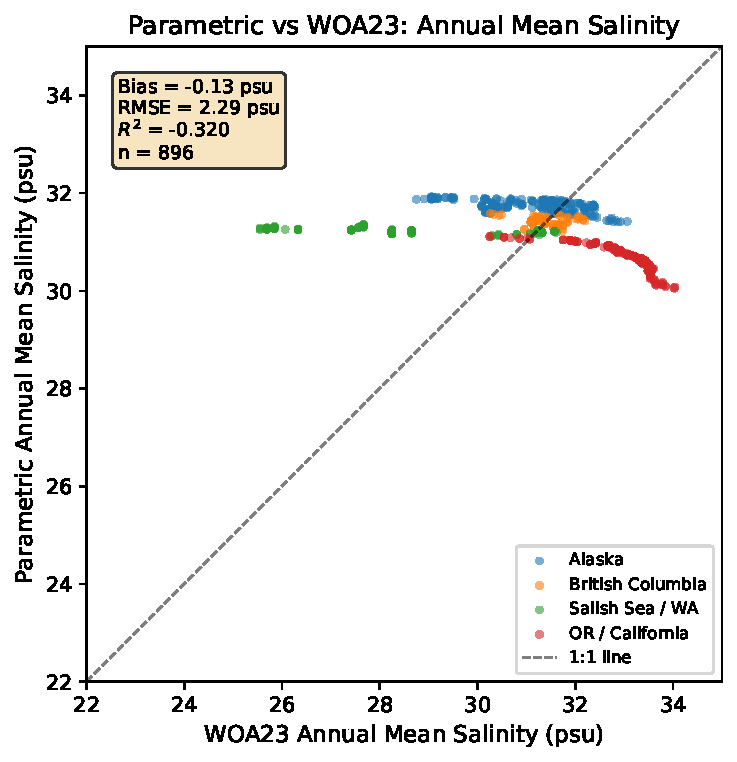
\includegraphics[width=0.75\textwidth]{fig1_scatter_annual.pdf}
    \caption{Parametric vs WOA23 annual mean salinity for 896 sites, coloured
    by region group. Dashed line: 1:1 agreement. The parametric model compresses
    a 12~psu WOA23 range into a $<$2~psu band. Bias $= -0.13$~psu,
    RMSE $= 2.29$~psu, $R^2 = -0.32$.}
    \label{fig:scatter}
\end{figure}

\subsection{Geographic Distribution of Bias}

Figure~\ref{fig:biasmap} maps the annual mean bias geographically. The spatial
structure is stark: strong negative bias (blue, parametric too low) dominates
California and Baja; strong positive bias (red, parametric too high) marks the
Salish Sea and Prince William Sound. The open coast of BC, Washington, and
western Alaska shows near-zero bias.

\begin{figure}[H]
    \centering
    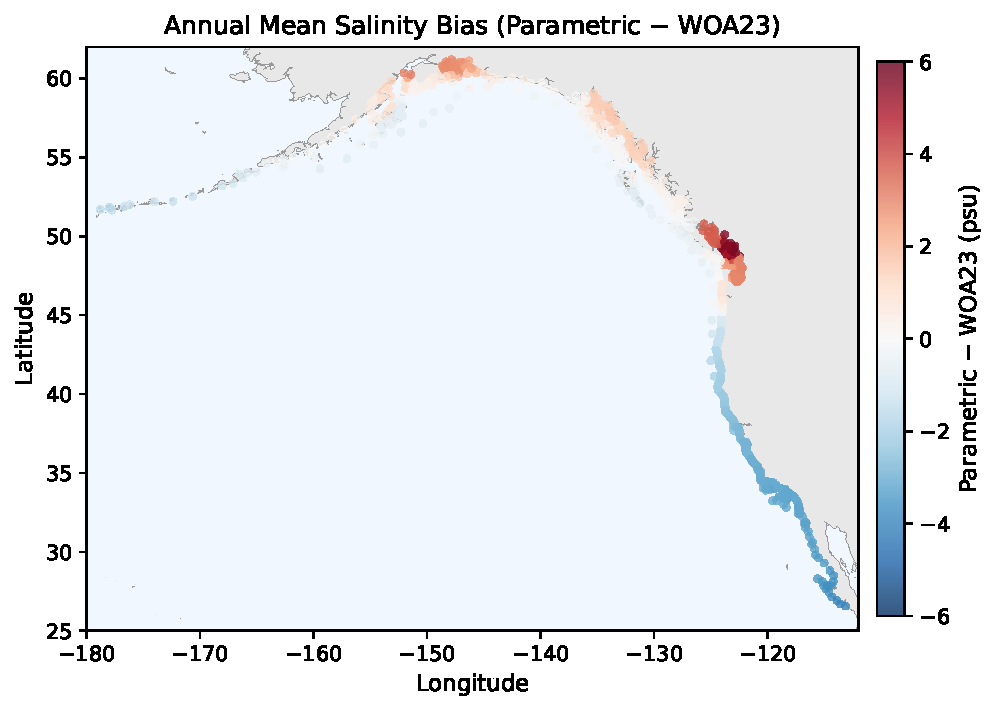
\includegraphics[width=0.75\textwidth]{fig2_bias_map.pdf}
    \caption{Geographic distribution of annual mean salinity bias (parametric
    $-$ WOA23). Blue: parametric underestimation; red: overestimation.
    Scale: $\pm$6~psu.}
    \label{fig:biasmap}
\end{figure}

\subsection{Regional RMSE Summary}

Table~\ref{tab:regions} summarises per-region statistics. The worst-performing
regions are SS-N (RMSE = 5.14~psu), SS-S (3.60~psu), BJ (3.46~psu), and
AK-PWS (3.21~psu). The best are AK-OC (0.37~psu), BC-N (0.53~psu), and
WA-O (0.60~psu).

\begin{table}[H]
\centering
\caption{Per-region comparison statistics, sorted by RMSE.}
\label{tab:regions}
\small
\begin{tabular}{lrrrrr}
\toprule
Region & $n$ & Bias (psu) & RMSE (psu) & WOA23 $\bar{S}$ & Seasonal Range \\
\midrule
AK-OC  & 28  & $+0.05$  & 0.37 & 31.66 & 0.97 \\
BC-N   & 75  & $+0.17$  & 0.53 & 31.28 & 1.09 \\
WA-O   & 36  & $+0.05$  & 0.60 & 31.14 & 1.46 \\
AK-EG  & 22  & $+0.27$  & 0.72 & 31.57 & 1.46 \\
BC-C   & 36  & $-0.06$  & 0.73 & 31.39 & 0.75 \\
AK-WG  & 79  & $+0.17$  & 0.94 & 31.57 & 1.22 \\
AK-AL  & 15  & $-1.12$  & 1.18 & 32.59 & 0.32 \\
AK-FS  & 48  & $+0.76$  & 1.25 & 30.87 & 2.08 \\
OR     & 59  & $-1.05$  & 1.39 & 32.04 & 1.35 \\
AK-FN  & 40  & $+1.12$  & 1.68 & 30.62 & 3.14 \\
CA-N   & 63  & $-2.20$  & 2.22 & 32.98 & 0.80 \\
JDF    & 26  & $+2.37$  & 2.69 & 28.84 & 2.11 \\
CA-C   & 97  & $-2.79$  & 2.80 & 33.39 & 0.38 \\
CA-S   & 78  & $-3.10$  & 3.10 & 33.54 & 0.19 \\
AK-PWS & 43  & $+2.29$  & 3.21 & 29.60 & 6.86 \\
BJ     & 31  & $-3.45$  & 3.46 & 33.67 & 0.25 \\
SS-S   & 89  & $+3.35$  & 3.60 & 27.87 & 2.95 \\
SS-N   & 31  & $+4.75$  & 5.14 & 26.55 & 4.93 \\
\bottomrule
\end{tabular}
\end{table}

% ===================================================================
% 4. SEASONAL DYNAMICS
% ===================================================================
\section{Seasonal Dynamics}

\subsection{The Missing Seasonal Cycle}

The most fundamental limitation of the parametric baseline is its complete
absence of seasonal variation. Every site receives the same salinity in January
as in August. In contrast, WOA23 reveals substantial seasonality: the mean
seasonal range across all 896 sites is 1.68~psu (median 1.04~psu), with
individual sites varying by up to 8.11~psu (Prince William Sound).

This matters for disease modelling because the salinity modifier
(Equation~\ref{eq:sal_mod}) is highly nonlinear near 28~psu. A site that
seasonally drops from 31~psu to 26~psu experiences meaningful transmission
suppression that the constant-baseline model cannot capture.

\subsection{Timing Heterogeneity}

Figure~\ref{fig:timing} maps the month of minimum WOA23 salinity geographically.
If all sites followed a simple summer-freshening pattern, minimum salinity would
be concentrated in June--August. Instead, the distribution is heterogeneous:

\begin{itemize}
    \item \textbf{May} --- 171 sites (19.1\%), the most common minimum month,
    driven by Alaska and BC sites responding to spring snowmelt.
    \item \textbf{June} --- 152 sites (17.0\%), peak river discharge in many
    northern regions.
    \item \textbf{February} --- 116 sites (12.9\%), dominated by OR/California
    where winter storms and increased river discharge drive fresher conditions.
    \item \textbf{August} --- 102 sites (11.4\%), capturing late-summer glacial
    melt in Prince William Sound and southeastern Alaska fjords.
\end{itemize}

The geographic map (Figure~\ref{fig:timing}) shows clear spatial coherence:
winter minima (blue tones) along California, spring minima (green--yellow) in
BC and western Alaska, and summer--autumn minima (orange--red) in the fjords
and Prince William Sound. This spatial pattern means the parametric model's
single June~15 melt pulse peak is at best a regional average, not a
site-appropriate timing.

\begin{figure}[H]
    \centering
    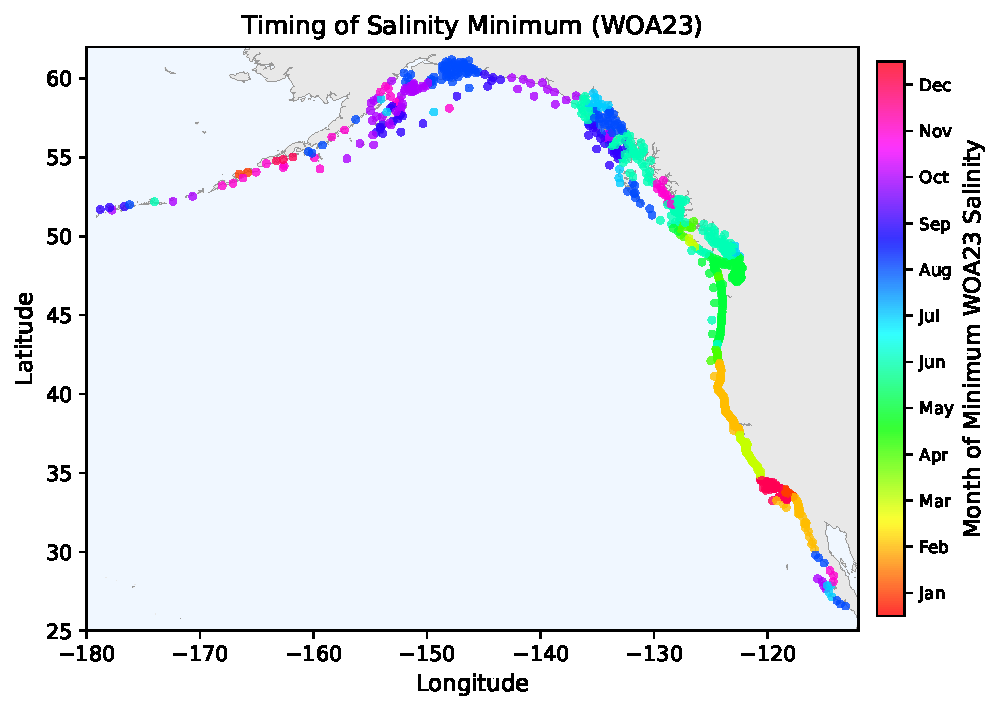
\includegraphics[width=0.75\textwidth]{fig3_timing_map.pdf}
    \caption{Month of minimum WOA23 salinity for each of the 896 sites.
    Colour encodes month (cyclic HSV scale). Winter minima dominate
    California; spring minima dominate BC; summer/autumn minima dominate
    Alaska fjords. The parametric model assumes a single June~15 peak
    everywhere.}
    \label{fig:timing}
\end{figure}

The stacked histogram in Figure~\ref{fig:timinghist} reinforces this pattern
quantitatively: salinity minima are distributed across nearly every month, with
no single month dominating. The regional colour coding reveals that winter
months (Dec--Feb) are dominated by OR/California sites, spring months (Mar--Jun)
by Alaska and BC, and late summer (Jul--Sep) by Alaska fjord sites. This
heterogeneity is fundamentally incompatible with a single-phase seasonal model.

\begin{figure}[H]
    \centering
    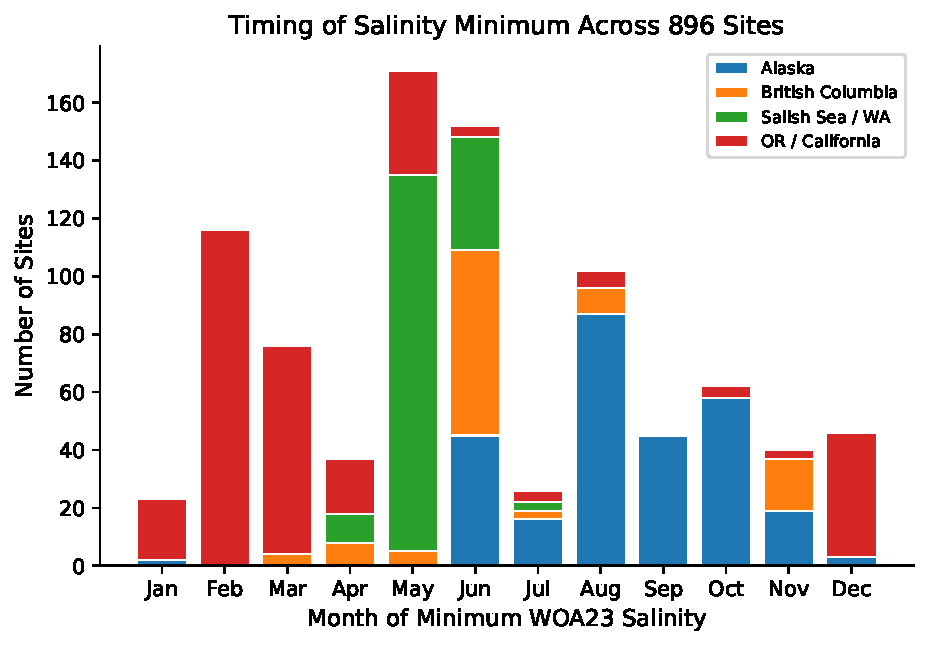
\includegraphics[width=0.85\textwidth]{fig3b_timing_hist.pdf}
    \caption{Stacked histogram of the month of minimum WOA23 salinity for 896
    sites, coloured by region group. No single month dominates; the four most
    common months are May (171), June (152), February (116), and August (102).}
    \label{fig:timinghist}
\end{figure}

\subsection{Seasonal Range Comparison}

Figure~\ref{fig:range} directly compares the seasonal range (max $-$ min monthly
salinity) between WOA23 and the parametric model. Panel~(a) shows the parametric
baseline (\texttt{fw\_strength=0}): every site has exactly zero seasonal range,
forming a horizontal line at $y=0$ while the WOA23 $x$-axis spans 0--8~psu.
Panel~(b) shows the parametric model with the melt pulse active
(\texttt{fw\_strength=15}), which introduces seasonality (mean range 3.93~psu)
but applies it only at high-latitude, high-enclosedness sites. Many California
and Oregon sites retain zero or near-zero parametric range despite WOA23 showing
non-trivial seasonal cycles there (0.2--1.4~psu from winter storms).

\begin{figure}[H]
    \centering
    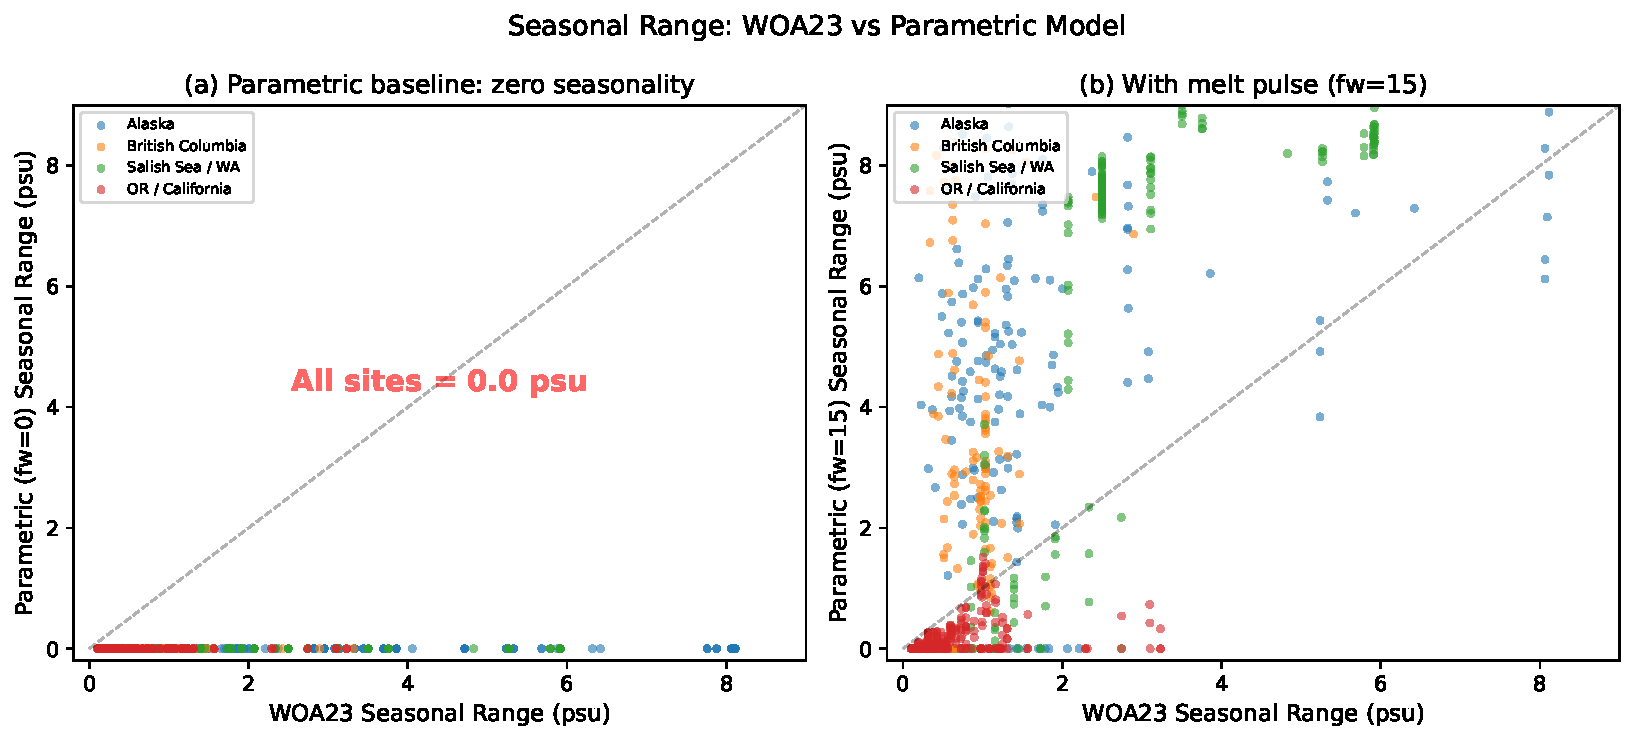
\includegraphics[width=\textwidth]{fig5_seasonal_range.pdf}
    \caption{Seasonal range comparison. (a) Parametric baseline
    (\texttt{fw\_strength=0}) has zero seasonal range at all sites.
    (b) With melt pulse (\texttt{fw\_strength=15}), Alaska sites gain
    seasonality but California/Oregon remain flat. WOA23 shows
    real seasonal cycles at all latitudes.}
    \label{fig:range}
\end{figure}

% ===================================================================
% 5. REGIONAL PROFILES
% ===================================================================
\section{Regional Profiles}

Figure~\ref{fig:profiles} presents mean seasonal profiles for each region group,
including the WOA23 10th--90th percentile envelope, the parametric baseline
(dashed), and the parametric model with melt pulse (\texttt{fw\_strength=15},
solid grey). DFO lighthouse observations appear as black circles in the BC panel.

Key regional observations:

\begin{itemize}
    \item \textbf{Alaska ($n=275$):} Strong spring--summer freshening
    (May--August), particularly in fjord regions (AK-FN: seasonal range
    3.14~psu, AK-PWS: 6.86~psu). The WOA23 10th--90th percentile shading
    spans 4--6~psu, showing high within-group heterogeneity. The parametric
    baseline sits near the upper bound of the WOA23 envelope. The melt pulse
    (fw=15) overshoots the WOA23 mean in summer because the cosine pulse
    applies the same timing (June~15) and amplitude scaling to all Alaska sites,
    while WOA23 shows earlier freshening in some subregions.

    \item \textbf{British Columbia ($n=111$):} Moderate seasonality
    ($\sim$1.0~psu mean range). The parametric baseline aligns well with the
    WOA23 mean year-round. DFO lighthouse data generally fall within the
    WOA23 envelope, validating both datasets in this region.

    \item \textbf{Salish Sea / WA ($n=182$):} The largest mismatch. WOA23 mean
    salinity is $\sim$28.4~psu (near the critical disease threshold), while
    the parametric model predicts $\sim$31.2~psu. The parametric model misses
    both the low mean and the 2.9~psu seasonal swing. Summer freshening drives
    WOA23 values to 26--27~psu in June--July, well into the suppression zone.

    \item \textbf{OR / California ($n=328$):} WOA23 sits at $\sim$33.1~psu
    year-round with modest winter freshening (February minimum, range
    0.58~psu). The parametric model runs $\sim$2.5~psu too low. Despite the
    small seasonal range, the consistent bias means the model systematically
    under-predicts the full-marine conditions that favour \textit{Vibrio}
    growth.
\end{itemize}

\begin{figure}[H]
    \centering
    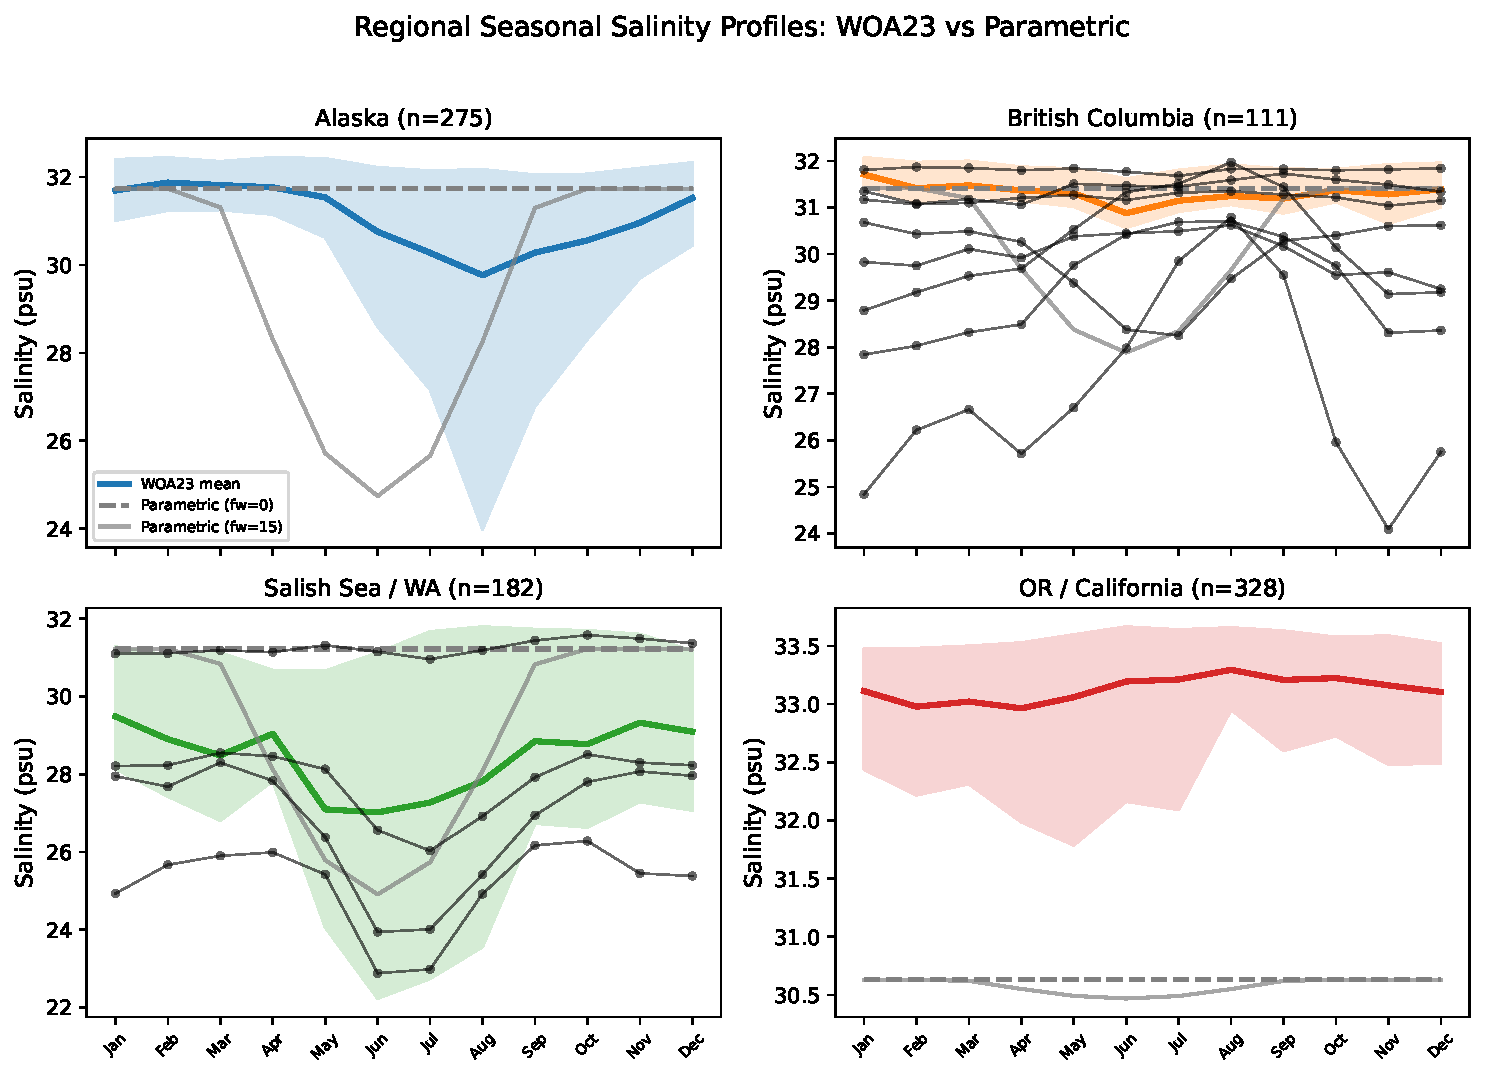
\includegraphics[width=\textwidth]{fig4_regional_profiles.pdf}
    \caption{Regional seasonal salinity profiles. Coloured line: WOA23 mean;
    shading: 10th--90th percentile range. Dashed grey: parametric baseline
    (fw=0). Solid grey: parametric with melt pulse (fw=15). Black circles:
    DFO lighthouse observations (visible in BC panels).}
    \label{fig:profiles}
\end{figure}

% ===================================================================
% 6. DATA QUALITY
% ===================================================================
\section{Data Quality}

Before drawing conclusions about the parametric model's performance, we must
assess the quality of the WOA23 benchmark itself. Two concerns are paramount:
the high fraction of sites requiring nearest-neighbour fill, and the accuracy
of WOA23 against independent in-situ observations.

\subsection{Nearest-Neighbour Fill Assessment}

Of the 896 sites, only 235 (26.2\%) fall within a WOA23 ocean grid cell. The
remaining 661 (73.8\%) required nearest-ocean-cell assignment. This high
proportion reflects the coastal and estuarine nature of the SSWD-EvoEpi
network --- rocky shores, fjord heads, and convoluted coastlines that lie
inside the 0.25\textdegree\ WOA23 land mask.

Figure~\ref{fig:nnmap} maps the extraction method for each site. The maximum NN
distance is 0.177\textdegree\ ($\approx$17~km), with a mean of
0.094\textdegree\ ($\approx$9~km). Most NN-filled sites are within one grid
cell of the coast. Sites with the largest NN distances are deep-fjord locations
where the nearest ocean cell represents open-coast conditions rather than
true fjord-head salinity.

\begin{figure}[H]
    \centering
    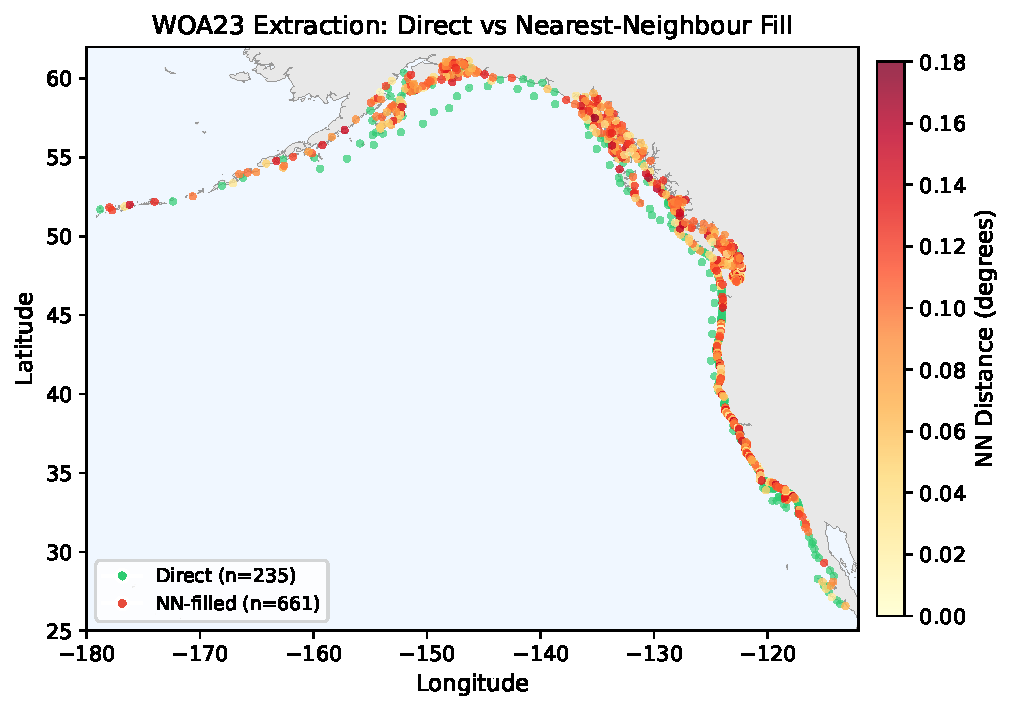
\includegraphics[width=0.75\textwidth]{fig6_nn_fill_map.pdf}
    \caption{WOA23 extraction method. Green: direct ocean cell (235 sites).
    Yellow--red gradient: NN-filled (661 sites), coloured by distance to
    nearest ocean cell (max 0.177\textdegree).}
    \label{fig:nnmap}
\end{figure}

\subsection{DFO Lighthouse Validation}

The 12 DFO lighthouse stations provide independent ground truth.
Figure~\ref{fig:dfo} shows monthly profiles for each station, comparing DFO
observations (black), WOA23 (blue), and parametric (red). Overall, WOA23
achieves a mean RMSE of 1.58~psu against DFO, compared to 2.26~psu for the
parametric model. The comparison is nuanced:

\begin{itemize}
    \item \textbf{Both models perform well:} Langara Island (WOA23 RMSE 0.28,
    parametric 0.27), Pine Island (0.25 vs 0.20), Bonilla Island (0.41 vs 0.33).
    These are exposed outer-coast stations with salinities near the parametric
    formula's calibration point.

    \item \textbf{WOA23 clearly wins:} Chrome Island (WOA23 0.72 vs parametric
    3.55), Departure Bay (1.51 vs 6.21), Entrance Island (1.26 vs 4.67).
    These Strait of Georgia stations have true salinities 4--6~psu below the
    parametric prediction. WOA23 captures the estuarine influence; the
    parametric formula cannot.

    \item \textbf{Both struggle:} Nootka Point (WOA23 5.02, parametric 4.73).
    This highly variable site with seasonal range $>$7~psu is poorly captured
    by both the 0.25\textdegree\ grid and the parametric formula.

    \item \textbf{Parametric wins:} Race Rocks (WOA23 2.67, parametric 0.18).
    Strong tidal mixing at this site produces salinities close to the open-ocean
    value captured by the formula, while WOA23's nearest ocean cell may be
    offset.
\end{itemize}

\begin{figure}[H]
    \centering
    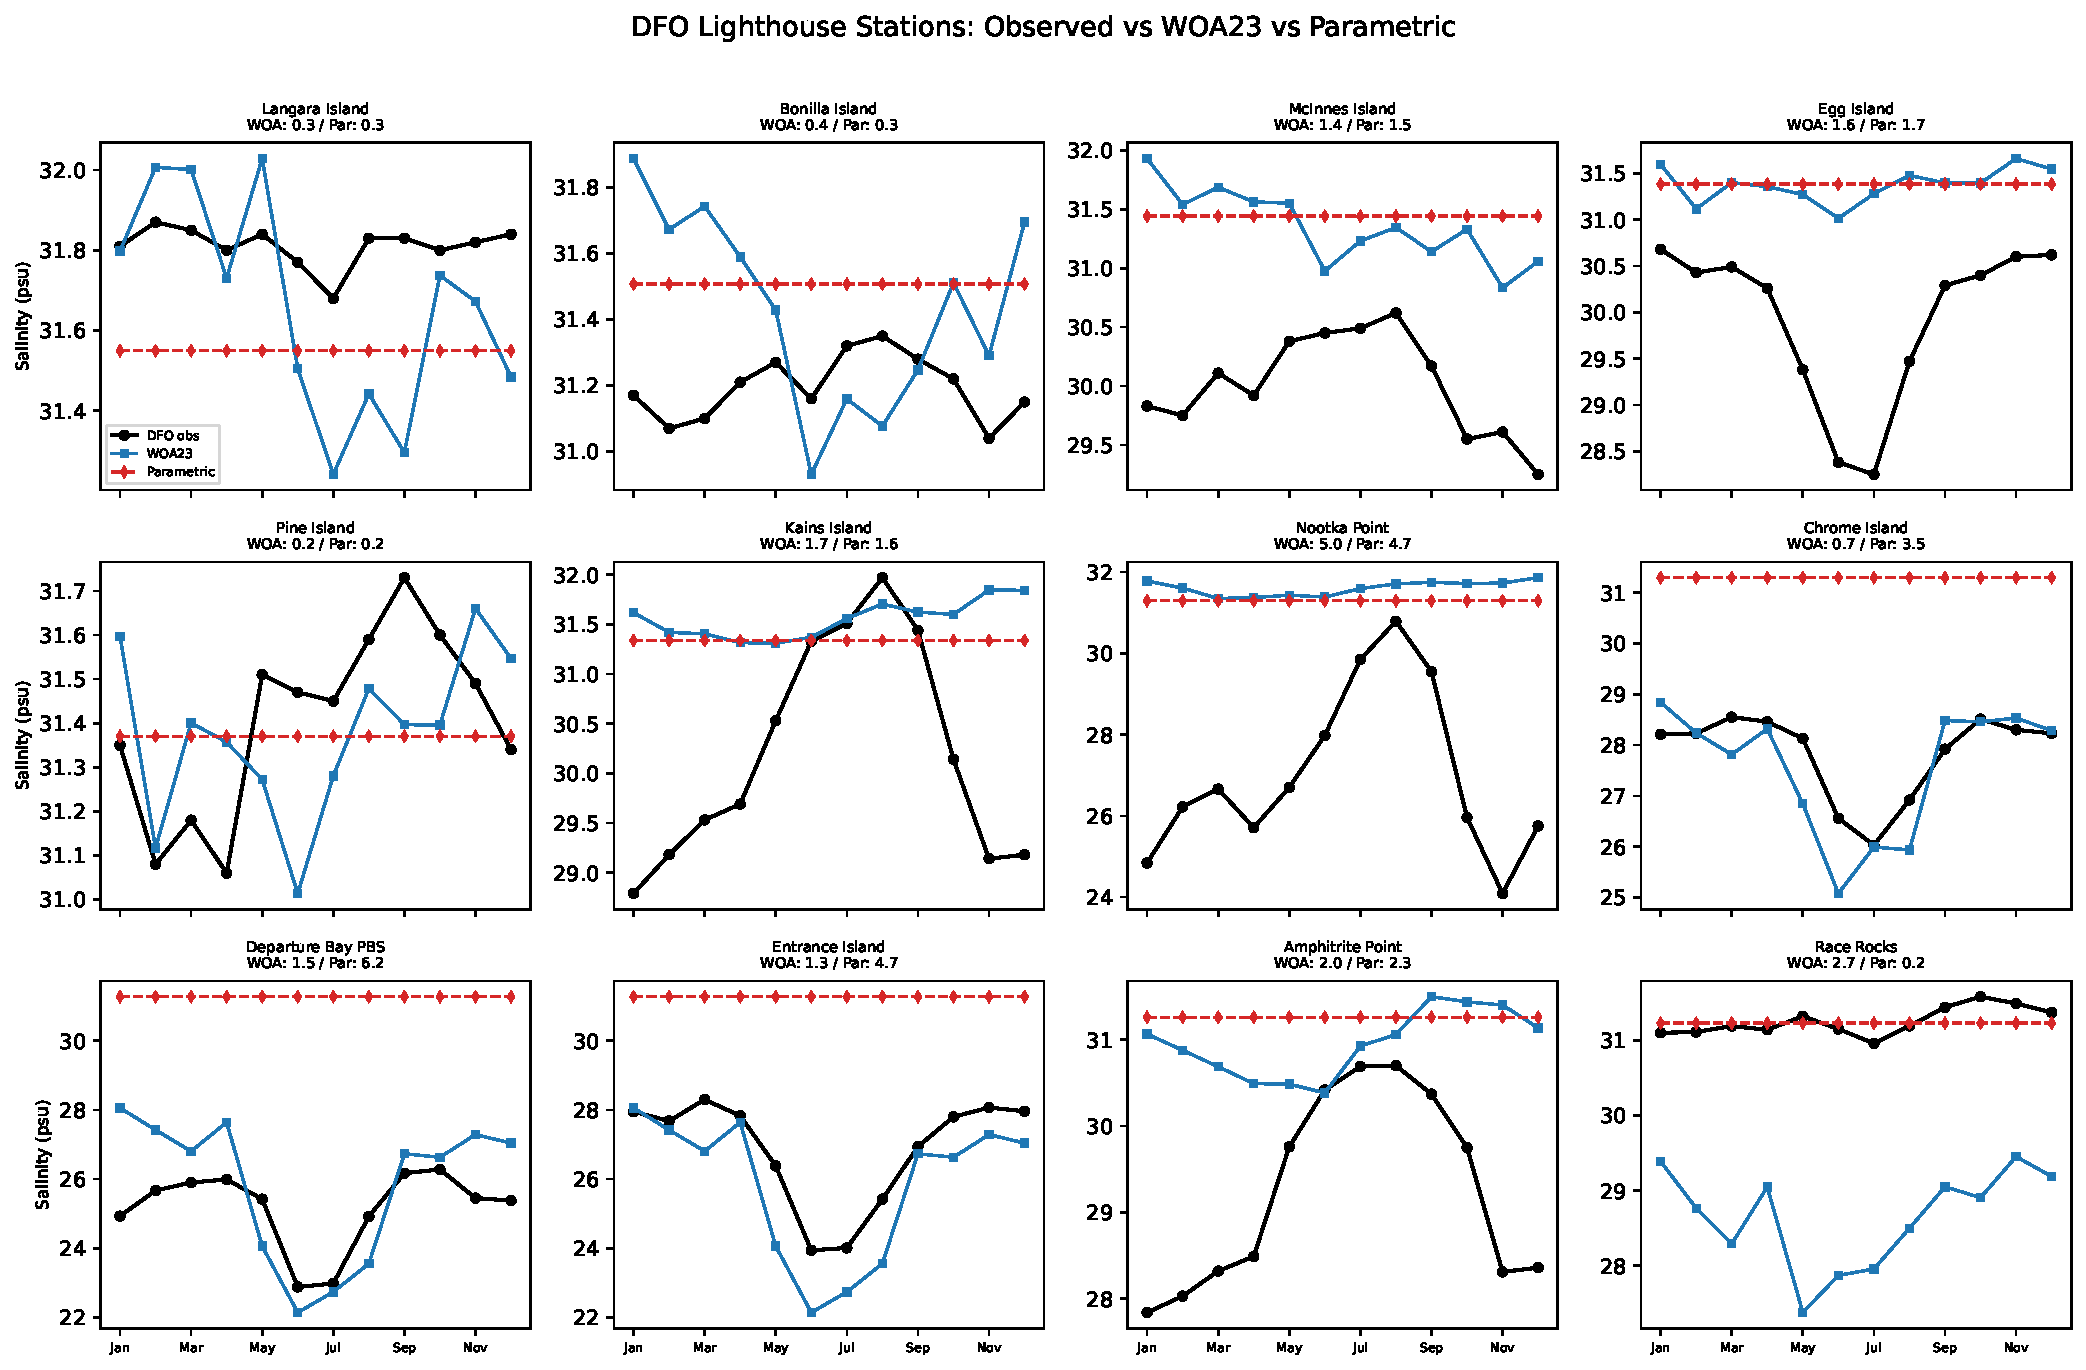
\includegraphics[width=\textwidth]{fig7_dfo_validation.pdf}
    \caption{Monthly salinity at 12 DFO lighthouse stations. Black circles:
    DFO observed climatology. Blue squares: WOA23. Red diamonds (dashed):
    parametric model. RMSE shown in each panel title (WOA23 / parametric).
    Mean RMSE: WOA23 = 1.58, parametric = 2.26~psu.}
    \label{fig:dfo}
\end{figure}

% ===================================================================
% 7. IMPLICATIONS FOR DISEASE MODEL
% ===================================================================
\section{Implications for Disease Modelling}

The preceding sections establish that the parametric model has large spatial
biases and no seasonal cycle. But do these errors actually matter for
disease predictions? This section translates salinity errors into disease
model outputs using the nonlinear salinity modifier
(Equation~\ref{eq:sal_mod}).

\subsection{Suppression Comparison}

Figure~\ref{fig:suppression} presents the most consequential comparison:
June disease transmission suppression under the parametric baseline versus
WOA23-informed salinity.

Under the \textbf{parametric baseline}, all 896 sites have June salinity
$>30$~psu, producing a salinity modifier of 1.0 everywhere. Zero sites
experience any suppression. The parametric model is entirely blind to
salinity-mediated disease dynamics.

Under \textbf{WOA23}, 143 sites show $>1\%$ transmission suppression.
The Salish Sea and Washington sites are most affected: mean suppression of
16.0\% (maximum 54.5\%), because WOA23 June salinity in this region averages
27.02~psu --- below the 28~psu threshold. This represents a qualitative
difference in model behaviour: the parametric model predicts full transmission
everywhere, while WOA23 reveals a substantial suppression zone in the most
ecologically sensitive region of the network.

\begin{figure}[H]
    \centering
    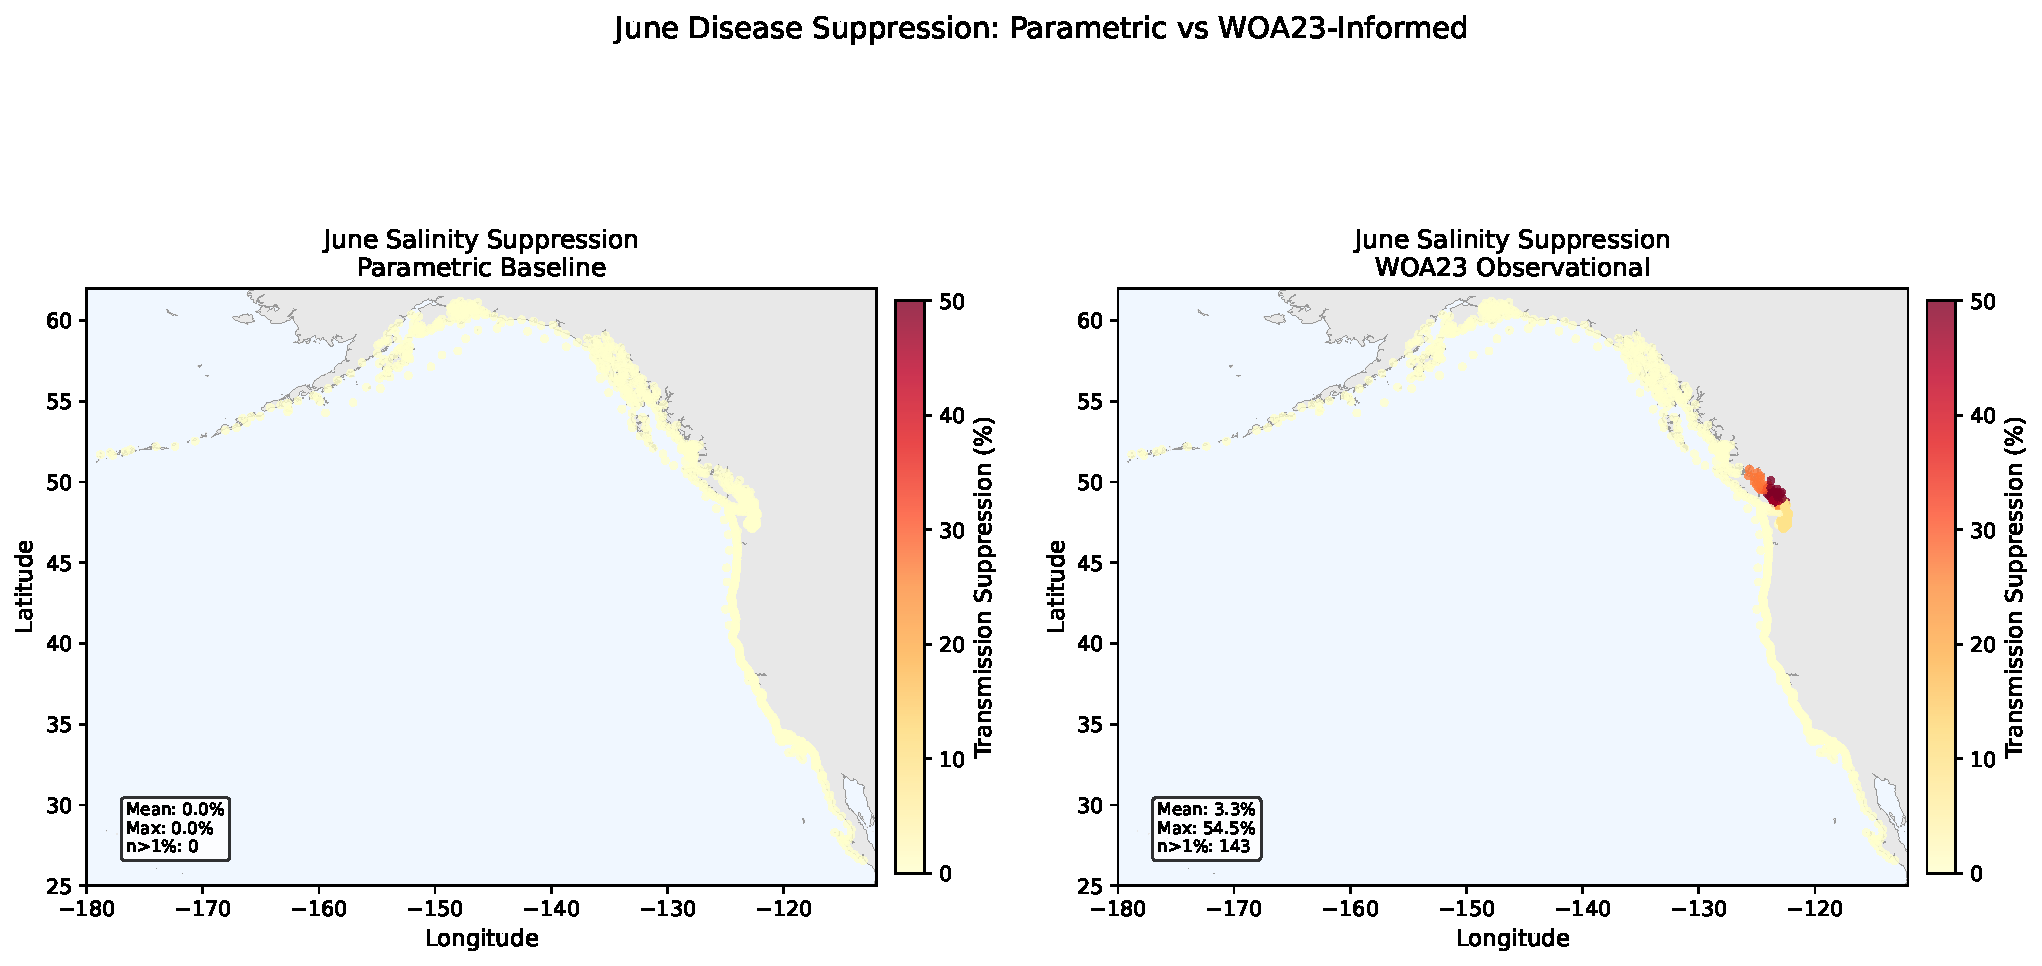
\includegraphics[width=\textwidth]{fig8_suppression_comparison.pdf}
    \caption{June transmission suppression (\%). Left: parametric baseline
    (0\% everywhere --- all sites above 30~psu). Right: WOA23 (up to 54.5\%
    suppression in the Salish Sea). The parametric model misses the entire
    suppression signal.}
    \label{fig:suppression}
\end{figure}

Table~\ref{tab:suppression} quantifies the regional suppression differences.
The Salish Sea is the critical region: the parametric model places it at
31.22~psu (full transmission), while WOA23 shows 27.02~psu (16\% mean
suppression). This 4.2~psu June bias directly translates to a qualitative
error in disease predictions for this region.

\begin{table}[H]
\centering
\caption{June salinity and disease suppression by region group.}
\label{tab:suppression}
\small
\begin{tabular}{lrrrr}
\toprule
Region & \multicolumn{2}{c}{June Salinity (psu)} & \multicolumn{2}{c}{Suppression (\%)} \\
\cmidrule(lr){2-3} \cmidrule(lr){4-5}
 & Parametric & WOA23 & Parametric & WOA23 \\
\midrule
Alaska          & 31.74 & 30.75 &  0.0 &  0.0 \\
British Columbia & 31.42 & 30.88 &  0.0 &  0.3 \\
Salish Sea / WA & 31.22 & 27.02 &  0.0 & 16.0 \\
OR / California & 30.63 & 33.19 &  0.0 &  0.0 \\
\bottomrule
\end{tabular}
\end{table}

\subsection{Latitude Gradient and the AK--CA Asymmetry}

Figure~\ref{fig:latgrad} shows the latitude--salinity relationship in June.
Panel~(a) reveals the real WOA23 pattern: June salinity is \emph{negatively}
correlated with latitude ($r = -0.46$), meaning high-latitude sites tend to
be \emph{fresher} in June due to snowmelt and glacial discharge. This is the
opposite of what one might naively expect from a simple ``colder = saltier''
assumption.

Panel~(b) shows the parametric model: a perfect positive linear relationship
($r = 1.0$) by construction, with all values compressed between 30.05 and
31.92~psu. The formula assumes higher-latitude sites are slightly saltier,
which is approximately true for annual means in open-ocean settings, but
becomes wrong in June when freshwater forcing is strongest.

Panel~(c) highlights the resulting bias pattern: the parametric model
overestimates June salinity at high latitudes (Alaska) and underestimates at
low latitudes (California). The two errors partially cancel in the global mean
bias, masking the regional pattern.

This asymmetry matters for the AK--CA disease comparison. The parametric model
predicts nearly identical salinity (and therefore transmission) across the
entire domain in June. WOA23 shows that Alaska sites are substantially
fresher, potentially experiencing salinity-mediated suppression that the
parametric model ignores, while California sites are substantially saltier,
experiencing full transmission that the parametric model also misrepresents.

\begin{figure}[H]
    \centering
    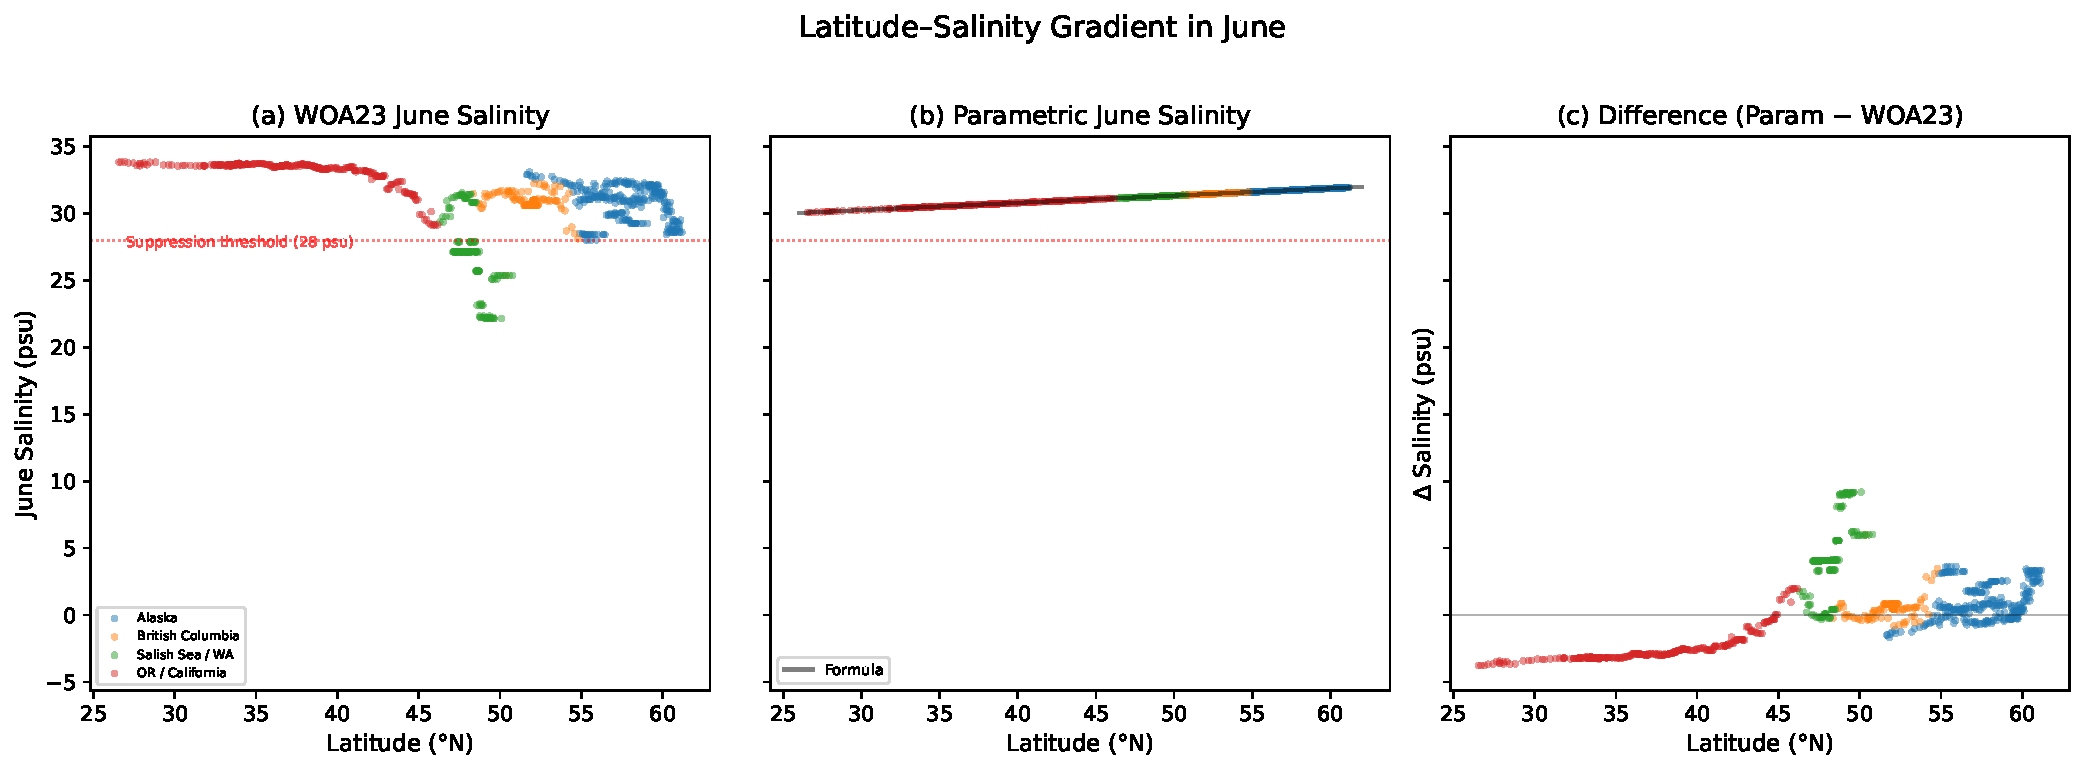
\includegraphics[width=\textwidth]{fig9_latitude_gradient.pdf}
    \caption{Latitude--salinity gradient in June. (a) WOA23: negative
    correlation ($r = -0.46$), higher latitudes fresher due to melt.
    (b) Parametric: perfect positive linear ($r = 1.0$) by construction.
    (c) Bias (parametric $-$ WOA23): systematic overestimation in Alaska,
    underestimation in California. Red dashed line at 28~psu indicates the
    disease suppression threshold.}
    \label{fig:latgrad}
\end{figure}

% ===================================================================
% 8. RECOMMENDATION
% ===================================================================
\section{Recommendation}

Based on this analysis, we recommend \textbf{replacing the parametric baseline
with WOA23 monthly climatology} as the default salinity input for the
SSWD-EvoEpi model. This change would:

\begin{enumerate}
    \item \textbf{Introduce site-specific seasonal cycles.} Mean seasonal range
    of 1.68~psu, capturing real freshwater forcing that the constant baseline
    ignores entirely.

    \item \textbf{Correct systematic regional biases.} The $+2.8$ to $+4.8$~psu
    overestimation in the Salish Sea --- where disease dynamics are most sensitive
    to salinity --- would be eliminated. The $-2.5$ to $-3.4$~psu
    underestimation along California would also be corrected.

    \item \textbf{Enable salinity-mediated suppression.} The 143 sites with
    $>1\%$ June suppression would gain this signal, particularly the 182
    Salish Sea/WA sites that currently show zero suppression.

    \item \textbf{Capture correct seasonal timing.} Winter-storm freshening in
    California (February minimum) and late-glacial melt in Alaska (August
    minimum) would be represented, rather than a universal June~15 pulse.

    \item \textbf{Reduce overall RMSE.} From 2.42~psu (parametric vs WOA23)
    to $\sim$1.58~psu (WOA23 intrinsic uncertainty vs DFO ground truth).
\end{enumerate}

\subsection{Implementation Notes}

The WOA23 monthly climatology for all 896 sites is already extracted and stored
as a $(896 \times 12)$ array. Integration requires:

\begin{itemize}
    \item Replacing the \texttt{ocean\_baseline(lat)} call with a lookup into
    the WOA23 monthly array for the current site and month.
    \item The existing \texttt{fw\_strength} mechanism could be applied \emph{on
    top of} the WOA23 baseline for sites where additional sub-grid freshwater
    forcing (fjord heads, river mouths) is needed, though the base WOA23 cycle
    already captures much of this variability.
    \item The WOA23 data file adds $<$100~KB to the model's data requirements.
\end{itemize}

\subsection{Caveats}

WOA23 is not without limitations:
\begin{itemize}
    \item \textbf{Resolution:} The 0.25\textdegree\ grid smooths over sub-grid
    features. Fjord-head sites may have surface salinity considerably lower than
    the nearest WOA23 ocean cell.
    \item \textbf{NN fill uncertainty:} 73.8\% of sites use NN-filled values.
    For deep-fjord sites, true salinity is likely lower than WOA23 due to
    unresolved river and glacial inputs.
    \item \textbf{Interannual variability:} WOA23 provides a long-term
    climatological mean, not year-specific conditions. Years with anomalous
    precipitation or snowmelt may deviate substantially.
    \item \textbf{Coastal accuracy:} The DFO validation shows RMSE of 1.58~psu
    against in-situ data, with individual stations reaching 5.02~psu (Nootka
    Point). WOA23 is an improvement, not ground truth.
\end{itemize}

Despite these limitations, WOA23 climatology represents a substantial
improvement over the parametric formula for all three dimensions of salinity
representation: spatial heterogeneity, seasonal dynamics, and absolute accuracy.

% ===================================================================
% 9. REFERENCES
% ===================================================================
\section*{References}

\begin{enumerate}
    \item Reagan, J. R., et al. (2024). World Ocean Atlas 2023.
    NOAA National Centers for Environmental Information.
    \item Fisheries and Oceans Canada. BC Lighthouse Sea-surface
    Temperature and Salinity Data.
    \item Eisenlord, M. E., et al. (2016). Ochre star mortality during the
    2014 wasting disease epizootic: role of population size structure and
    temperature. \textit{Philosophical Transactions of the Royal Society B},
    371(1689), 20150212.
\end{enumerate}

\end{document}
